\documentclass[a4paper,twocolumn]{article}
\usepackage[landscape]{geometry}
\usepackage{graphicx} % Required for inserting images
\usepackage[f]{esvect}
\usepackage{mathtools}
\usepackage{enumitem}
\usepackage{siunitx}
\sisetup{input-digits = 0123456789\pi}
\usepackage{hyperref}
\usepackage{float}

\newcommand{\dive}[1]{\mathrm{div}\left( #1 \right)}
\newcommand{\rota}[1]{\vv{\mathrm{rot}}\left( #1 \right)}

\geometry{%
  a4paper,                % format de papier
% Définition des marges :
  left= 2.5cm,            % marge intérieure à la page
  right = 2.5cm,          % marge extérieure
  top = 2cm,
  bottom = 2cm,
% En-tête et pied de page :
  headheight=6mm,         % espace réservé à l'en-tête dans la marge top
  %headsep=3mm,            % espace entre le corps et l'en-tête
  %footskip=9mm            % espace entre le corps et le pied de page
}

\begin{document}


\section*{TD1}

\begin{center}
    \large\bf Raisonner simplement, convertir
  \end{center}
  
\subsubsection*{Exercice 1} 

\begin{enumerate}
	\item On considère la marche d'une kinésine le long d'un microtubule, qui se fait à vitesse moyenne de $\langle v \rangle =\SI{1.8}{\nano\meter\per\second}$. Au bout de quelle durée cette kinésine aura-t-elle traversé de bout en bout un microtubule de longueur $L=\SI{0.04}{\micro\meter}$ ?
	\item Une cellule migre à une vitesse constante de $v_0=\SI{5}{\micro\meter\per\minute}$. En supposant le mouvement rectiligne, donner la distance parcourue par la cellule au bout de $\SI{2}{\hour}$. On donnera la réponse en millimètres.
\end{enumerate}

  \begin{center}
    \large\bf Décrire un mouvement
  \end{center}

\subsubsection*{Exercice 2} 

\begin{figure}[H]
	\centering
	\includegraphics[width=0.8\linewidth]{reperage.pdf}
\end{figure}

\begin{enumerate}
	\item Exprimer les coordonnées cartésiennes des points ci-dessus puis écrire le vecteur position $\vv{OM}$ associé. Tracer les vecteurs unitaires de la base cartésienne, attachés au point $M$. La base cartésienne est-elle une base fixe ou mobile ?
	\item Mêmes questions avec les coordonnées et la base polaires. \textit{On pourra utiliser les fonctions tangente et arctangente pour le cas c)}
	
	\item Calculer le vecteur déplacement associé aux trajectoires suivantes. En considérant que les trajets ont été faits sur une durée $\Delta t = \SI{5}{\second}$, en déduire le vecteur vitesse moyenne associé (on prendra le mètre comme unité des axes).
\end{enumerate}

\begin{figure}[H]
	\centering
	\includegraphics[width=0.8\linewidth]{trajectoires.pdf}
\end{figure}

\subsubsection*{Exercice 3} 

\begin{enumerate}
	\item Donner les dérivées des fonctions suivantes :
	
	\begin{equation*}
	f(x) = x^2+\frac{1}{x}, \quad g(t) = A\cos (\omega t), \quad h(y) = y^2\exp (-ay)
	\end{equation*}
	
	\item Donner une primitive des fonctions suivantes :
	
	\begin{equation*}
	f(x) = 3x^2+2, \quad g(t) = t+\cos(t), \quad h(y) = (2-ay)ye^{-ay}
	\end{equation*}
	
	\noindent Donner les primitives de ces mêmes fonctions qui s'annulent en $x=1$ (pour $f$), $t=-1$ (pour $g$) et $y=0$ (pour $h$).

	\item On donne les vecteurs position suivants. Calculer les vecteurs vitesse et accélération associés.
	
	\begin{equation*}
		\vv{OM}(t) = v_0 t\vv{e_x} + \left(y_0+\frac{1}{2}a_0t^2\right) \vv{e_y}, \quad \vv{OM}(t) = A\cos (\omega t)\vv{e_x} + A\sin(\omega t)\vv{e_y}
	\end{equation*}
	
	\item On donne le vecteur accélération suivant : $\vv{a} = -g\vv{e_z}$. En supposant les conditions initiales $\vv{OM}(t=0) =h\vv{e_z}$ et $\vv{v}(t=0)=v_0\vv{e_y}$, calculer les vecteurs vitesse et position associés. Pour quelle valeur de $t$ a-t-on $z=0$ ?
	
\end{enumerate}

\subsubsection*{Exercice 4} 

On donne les équations horaires décrivant le mouvement d'un grain de sable en sédimentation dans l'eau :
	
	\begin{equation*}
		x(t) = x_0+\tau v_0\left( 1-e^{-t/\tau} \right),\quad y(t)=a_0\tau^2\left( 1-e^{-t/\tau}-\frac{t}{\tau} \right)
	\end{equation*}

\begin{enumerate}

	\item Écrire le vecteur position associé au grain de sable à tout instant $t$.	
	
	\item Calculer la vitesse et l'accélération du grain de sable à tout instant $t$.
	
	\item Déterminer l'équation de la trajectoire $y(x)$. En déduire la profondeur $y$ du grain de sable lorsqu'il atteint la position $x=0$. Faire l'application numérique pour $v_0 = \SI{36}{\milli\meter\per\minute}$, $x_0=\SI{1}{\cm}$, $\tau=\SI{0.5}{\second}$ et $a_0=\SI{35000}{\meter\per\minute\squared}$
	
\end{enumerate}

\subsubsection*{Exercice 5} 

\begin{figure}[h]
	\centering
	\includegraphics[width=0.6\linewidth]{araignee.pdf}
\end{figure}

On considère une araignée de masse $m$ se balançant, suspendue au bout d'un fil de longueur $l$. Les équations horaires du mouvement de l'araignée sont :

\begin{equation*}
	x(t) = x_0\cos(\omega t), \quad y(t) = y_0 + \frac{l}{2}\left( \cos(2\omega t) - 1 \right)
\end{equation*}

\begin{enumerate}
	\item Écrire le vecteur position de l'araignée à tout instant $t$.
	\item En déduire le vecteur vitesse instantané associé.
	\item Pour quelles positions la vitesse de l'	araignée s'annule-t-elle ?
	\item Calculer l'accélération de l'araignée au bout du pendule à chaque instant $t$.
	\item Bonus : Reprendre les questions suivantes en utilisant un repère polaire et les équations horaires :
	
	\begin{equation*}
	r(t) = l, \quad \theta(t) = \theta_0\cos (\omega t)
\end{equation*}
	
\end{enumerate}

\subsubsection*{Exercice 6 (tiré de Physique tout-en-un PCSI, Dunod)}

Dans un épisode de la Star Wars, on
peut assister à une course poursuite de speeder entre des cheminées d’usine. On suppose que le véhicule suit une trajectoire sinusoïdale de slalom entre les cheminées alignées selon l’axe $(Ox)$. Elles sont espacées d’une distance $L = \SI{200}{\meter}$.

\begin{figure}[h]
	\centering
	\includegraphics[width=0.4\linewidth]{chem.png}
\end{figure}

\begin{enumerate}
	\item Le véhicule conserve une vitesse $v_0$ constante selon $(Ox)$ et met $t_t = \SI{12}{\s}$ pour revenir sur l’axe après la sixième cheminée. En déduire la vitesse $v_0$. Faire l’application numérique.
	\item Déterminer l’amplitude de la sinusoïde pour que l’accélération reste inférieure à $10g$ en
valeur absolue, avec $g = \SI{9,8}{\meter\per\second\squared}$ . Que penser des valeurs obtenues ?
\end{enumerate}

\newpage

\section*{TD2}

\begin{center}
    \large\bf Raisonner simplement
  \end{center}
  
  Mini exercice pour faire comprendre pk des trucs flottent ou pas.

  \begin{center}
    \large\bf Poser un problème de dynamique
  \end{center}
  
  \subsubsection*{Exercice 1}
  
  On dépose un échantillon de sang de masse volumique $\rho_s$ et de viscosité $\eta_s$ dans un tube à essai et on observe la sédimentation rectiligne d'un globule rouge vers le fond du tube, ce premier était assimilé à une sphère de rayon $R$ et de masse volumique $\rho$. On note $\vv{g}$ l'accélération de la pesanteur.
  
  \begin{enumerate}
  	\item Définir un repère adapté à l'étude de ce mouvement et faire un schéma du système.
  	\item Quelles sont les forces s'appliquant sur le globule rouge ? Quelles sont leur expression littérale ? Les tracer sur le schéma.
  \end{enumerate}
  
  \subsubsection*{Exercice 2}
  
  On considère un noyau cellulaire plongé dans le cytoplasme, piégé par une pince optique modélisée par un ressort de raideur $k$.
  
  \begin{enumerate}
  	\item Définir un repère adapté à l'étude de ce mouvement et faire un schéma du système.
  	\item Quelles sont les forces s'appliquant sur le noyau ? En introduisant les grandeurs nécessaires donner leur expression littérale ? Les tracer sur le schéma.
  \end{enumerate}
  
  \begin{center}
    \large\bf Déterminer une trajectoire
  \end{center}
  
 \subsubsection*{Exercice 3}
 
 \paragraph{}On considère une protéine de charge nette $q$ que l'on fait migrer par électrophorèse le long d'une ligne de gel dirigée par le vecteur unitaire $\vv{e_x}$. Pour ce faire, on applique dans le gel un champ électrique uniforme $\vv{E}=E_0\vv{e_x}$. On considère que la protéine est initialement à la position $x=0$ et possède une vitesse nulle.
 
 \begin{enumerate}
 	\item Écrire le PFD appliqué à la protéine en supposant que la force de Coulomb est la seule force en jeu.
 	\item Intégrer l'équation obtenue pour obtenir le vecteur position à tout temps. À quel instant $t_1$ la protéine atteint-elle le bout du gel en $x=L$ ?
\end{enumerate}  
 
\paragraph{}En réalité, lors de la migration dans le gel, la protéine est soumise à une force de frottements fluides qui finit par conférer à la protéine une vitesse limite de migration constante.

 \begin{enumerate}[resume]
 	\item Écrire le PFD en considérant cette nouvelle force. On notera $\eta$ la viscosité du gel et $R$ le rayon hydrodynamique de la protéine.
 	\item En déduire la vitesse limite de migration de la protéine.
 	\item On met au début de la ligne de gel un mélange de protéines de charge nette $q$ et de protéines de charge nette $2q$. Expliquer comment cette méthode peut-elle permettre de séparer les différents constituants du mélange.
\end{enumerate} 
  
  \begin{center}
    \large\bf Caractériser une force
  \end{center}

\paragraph{Exercice 4}

\paragraph{}On attache au bout d'une kinésine une bille que l'on piège dans une pince optique. La zone de focalisation de la pince optique se trouve en $x=0$ et la force qu'elle exerce sur la bille est modélisée par un ressort de raideur $k$. D'autre part, la kinésine exerce une force de traction constante $\vv{F}=F_0\vv{e_x}$ qui l'éloigne du centre de la pince optique.

\begin{enumerate}
	\item Faire un schéma simplifié de la situation.
	\item Écrire le PFD appliqué à la bille.
\end{enumerate}

\paragraph{}Après un court instant, la bille se stabilise à la position $x_0$.

\begin{enumerate}[resume]
	\item En déduire la force exercée par le moteur moléculaire sur la bille.
\end{enumerate}

  \begin{center}
    \large\bf Résoudre des problèmes
  \end{center}

exo sur la méthode BACS

\newpage

\section*{TD3}

\begin{center}
    \large\bf Calculer des travaux et une puissance
  \end{center}
  
  \begin{center}
    \large\bf Utiliser le théorème de l'énergie cinétique
  \end{center}
  
  \begin{center}
    \large\bf Calculer une force à partir d'une énergie potentielle
  \end{center}
  
  \begin{center}
    \large\bf Utiliser le principe de conservation de l'énergie mécanique
  \end{center}

\paragraph{} On étudie la propagation d'une OEM dans le vide.

\begin{enumerate}
    \item Rappeler l'équation aux dérivées partielles à laquelle satisfont les champs $\vv{E}$ et $\vv{B}$.
\end{enumerate}

\begin{enumerate}[resume]
\item On suppose que le champ électrique est de la forme :

\begin{equation*}
    \vv{E} = E_0\cos(\omega t - kz)\hat{e}_x, \quad k, \omega>0
\end{equation*}
\begin{enumerate}
    \item A quelle équation doit satisfaire $k$ pour que ce champ soit solution de l'équation précédemment citée ?
    \item Quels sont la direction, le sens et la vitesse de propagation de cette onde ?
    \item Quelle est la structure de cette onde ?
    \item Calculer le champ magnétique $\vv{B}$ associé à $\vv{E}$ ainsi que le vecteur de Poynting de l'onde ?
\end{enumerate}

\item La puissance moyenne rayonnée par cette onde à travers une surface $S=\SI{4}{\milli\meter\squared}$ orthogonale à sa direction de propagation est $P=\SI{10}{\watt}$. Calculer les amplitudes $E_0$ et $B_0$ des champs électriques et magnétiques. On donne $\mu_0 =\SI{4\pi e-7}{\henry\per\meter}$.

\end{enumerate}

\begin{center}
    \large\bf Onde électromagnétique plane progressive 2
  \end{center}

\paragraph{}On étudie une onde électromagnétique dont le champ électrique est :

\begin{equation*}
    \underline{\vv{E}} = \underline{E_x} \hat{e}_x + \underline{E_y} \hat{e}_y \quad \text{avec} \quad \underline{E_x} = E_0\exp\left( i \left(\omega t -  \frac{K}{3}(2x+2y+z) \right) \right)
\end{equation*}

\noindent L'onde se propage dans le vide et sa longueur d'onde est $\lambda = \SI{6e-7}{\meter}$.

\begin{enumerate}
    \item Calculer la fréquence de l'onde.
    \item Dans quel domaine du spectre électromagnétique se situe cette onde ?
    \item Exprimer le vecteur d'onde en fonction de $K$.
    \item Calculer la valeur numérique de la constante $K$.
    \item Établir l'équation cartésienne d'un plan d'onde.
    \item Exprimer $\underline{E_y}$ en fonction de $\underline{E_x}$ en utilisant l'équation de Maxwell-Gauss dans la représentation complexe.
    \item Calculer le champ magnétique $\underline{\vv{B}}$ associé à cette onde.
    \item Calculer la densité moyenne d'énergie électromagnétique associée à cette onde.
    \item Calculer le vecteur de Poynting de cette onde et sa moyenne temporelle. 
\end{enumerate}

\begin{center}
    \large\bf Communication avec la Terre (E3A MP 2015)
  \end{center}

\paragraph{} On se propose d'étudier la propagation des ondes électromagnétiques entre la sonde Rosetta et la Terre, dans le vide.

\begin{enumerate}
    \item Rappeler les équations de Maxwell en présence de charges et de courants. Comment se simplifient-elles dans le vide ?
    \item Etablir l'équation de propagation dans le vide vérifiée par le champ électrique $\vv{E}$. Donnez celle vérifiée par le champ magnétique $\vv{B}$.
    \item En déduire la célérité des ondes électromagnétiques dans le vide en fonction de $\mu_0$ et $\epsilon_0$.
\end{enumerate}

\noindent On considère une onde électromagnétique pour laquelle le champ électrique en coordonnées cartésiennes s'écrit :

\begin{equation*}
    \vv{E}(z,t) = E_x\cos\left( \omega \left( t-\frac{z}{c} \right) \right)\hat{e}_x + E_y\cos\left( \omega \left( t-\frac{z}{c} \right) \right)\hat{e}_y + E_z\cos\left( \omega \left( t-\frac{z}{c} \right) \right)\hat{e}_z
\end{equation*}

\noindent où $E_x$, $E_y$ et $E_z$ sont des constantes.

\begin{enumerate}[resume]
    \item Dans quelle direction se propage cette onde ? Est-ce une OPPH ? Exprimer son vecteur d'onde $k$.
    \item Simplifier l'expression donnée du champ électrique à l'aide de l'équation de Maxwell-Gauss.
\end{enumerate}

\noindent Le champ magnétique associé s'écrit :

\begin{equation*}
    \vv{B}(z,t) = B_x\cos\left( \omega \left( t-\frac{z}{c} \right) \right)\hat{e}_x + B_y\cos\left( \omega \left( t-\frac{z}{c} \right) \right)\hat{e}_y + B_z\cos\left( \omega \left( t-\frac{z}{c} \right) \right)\hat{e}_z
\end{equation*}

\noindent où $B_x$, $B_y$ et $B_z$ sont des constantes.

\begin{enumerate}[resume]
    \item Déterminer $B_x$, $B_y$ et $B_z$ en fonction de $E_x$, $E_y$ et $c$.
    \item Cette onde est-elle transversale ou longitudinale par rapport à la direction de propagation ?
\end{enumerate}

\begin{center}
    \large\bf Ondes sphériques
  \end{center}

\paragraph{}On considère un émetteur isotrope d'ondes électromagnétiques que l'on assimile à une source ponctuelle : il peut s'agir d'un émetteur de radio, d'un satellite, d'une étoile qui rayonne, etc. L'onde émise est sphérique, de la forme en coordonnées sphériques :
$$
\vv{E}(\vv{r}, t)=E_0(r) \cos (\omega t-k r) \hat{e}_\theta \quad \text { avec } \quad k=\frac{\omega}{c} .
$$

\noindent Le milieu de propagation est assimilé au vide.

\begin{enumerate}
    \item Par analogie avec une onde plane, identifier le vecteur d'onde $\vec{k}$ de l'onde sphérique.
    \item On admet qu'une telle onde vérifie localement la même relation de structure qu'une onde plane. En déduire l'expression du champ magnétique associé.
    \item Exprimer le vecteur de Poynting et sa moyenne temporelle.
    \item Exprimer la puissance moyenne $\mathcal{P}$ rayonnée à travers une sphère de rayon $r$. Justifier par un argument physique que cette puissance est indépendante de $r$. En déduire que $E_0(r)=A / r$ avec $A$ une constante à déterminer.
\end{enumerate}

  \begin{center}
    \large\bf Mesures de concentration en CO$_2$ dans l'atmosphère (DS 2023)
  \end{center}

  \paragraph{}Le développement de modèles climatiques et l’actualisation de leurs prédictions nécessitent des mesures précises
de la fraction molaire en CO$_2$ présent dans l’atmosphère. Celle-ci est usuellement exprimée en parties par millions
(ppm) : une fraction molaire de 413 ppm indique par exemple qu’un million de molécules d’air contient en moyenne
413 molécules de CO$_2$.
\paragraph{}Pour ce faire, un échantillon d’air est prélevé, de préférence en relative altitude et loin de toute perturbation
humaine, puis refroidi pour condenser toute la vapeur d’eau, avant d’être analysé. Le principe est celui de la spectrophotométrie : un faisceau laser de longueur d’onde $\SI{4.26}{\micro\meter}$, à laquelle le spectre d’absorption du CO$_2$ présente un
maximum, traverse un échantillon de longueur connue. Comparer les intensités lumineuses avant et après traversée
de l’échantillon permet d’en déduire la concentration en CO$_2$, en nombre de molécules par $\text{m}^3$ d’air. Les capteurs
de CO$_2$ popularisés comme indicateurs de la qualité de l’air lors de la crise du Covid-19 fonctionnent sur le même
principe mais avec des exigences de précision bien moindre.

\begin{figure}[h]
    \centering
    \includegraphics[width=0.6\linewidth]{SchemaAbsorption.pdf}
    \caption{Principe de fonctionnement de la mesure}
    \label{fig:enter-label}
\end{figure}

\begin{enumerate}
    \item On modélise le faisceau laser par un cylindre de section $S$ au sein duquel se propage dans la direction $+\hat{e}_z$ une onde plane progressive
harmonique polarisée rectilignement selon $\hat{e}_x$. 

\begin{enumerate}
    \item Écrire le champ électrique $\vv{E}(\vv{r},t)$ associé à cette onde. On notera $E_0$ son amplitude, $\omega$ sa pulsation et $k$ la norme de son vecteur d'onde.
    \item En déduire le champ magnétique $\vv{B}(\vv{r},t)$  associé.
    \item En déduire le vecteur de Poynting $\vv{\Pi}(\vv{r},t)$ associé ainsi que sa moyenne temporelle $\langle\vv{\Pi}(\vv{r},t)\rangle$ et son intensité $I = \lVert \langle\vv{\Pi}(\vv{r},t)\rangle\rVert$.
\end{enumerate}

\item Dans l'échantillon, l'onde interagit avec la matière. On suppose alors que cette première conserve la même structure mais que la quantité d'énergie qu'elle transporte dépend maintenant de son avancée dans l'échantillon :

\begin{equation*}
    \langle\vv{\Pi}(\vv{r},t)\rangle = I(z)\hat{e}_z
\end{equation*}


\noindent avec $I(z)$ l'intensité du faisceau en $z$. 

\paragraph{}Chaque molécule de CO$_2$ se trouvant dans le faisceau absorbe en moyenne une puissance $p$ proportionnelle à l’intensité : $p = \sigma I$, où $\sigma$ est une constante tabulée dépendant uniquement de la longueur d’onde. On se propose de raisonner sur une tranche infinitésimale du faisceau située entre $z$ et $z+\mathrm{d}z$ pour déterminer la loi d'évolution de l'intensité $I(z)$ au cours de la traversée de l'échantillon.

\begin{figure}[h]
    \centering
    \includegraphics[width=0.4\linewidth]{BilanTranche.pdf}
    \caption{Tranche infinitésimale du faisceau située entre $z$ et $z+\mathrm{d}z$}
\end{figure}

\begin{enumerate}
    \item Quelle est la dimension de $\sigma$ ?
    \item Exprimer la puissance moyenne $\mathcal{P}(z)$ transmise par l'onde à travers la surface $S$ à l'abscisse $z$ en fonction de $I(z)$ et $S$. De même, exprimer la puissance moyenne $\mathcal{P}(z+\mathrm{d}z)$ transmise par l'onde à travers la surface $S$ à l'abscisse $z+\mathrm{d}z$.
    \item On note $n$ la densité volumique de CO$_2$, c’est-à-dire le nombre de molécules de CO$_2$ par unité de volume dans l’échantillon. Déterminer la puissance moyenne totale absorbée $\mathrm{d}P_\text{abs}(z)$ par les molécules de CO$_2$ dans cette tranche en fonction de $n$, $\sigma$, $S$, $\mathrm{d}z$ et $I(z)$.
    \item En le justifiant par un argument de conservation de l'énergie, déterminer une relation entre $\mathcal{P}(z)$, $\mathcal{P}(z+\mathrm{d}z)$ et $\mathrm{d}P_\text{abs}(z)$
    \item En déduire que l'intensité du faisceau vérifie l'équation différentielle :

    \begin{equation*}
        \frac{\mathrm{d}I}{\mathrm{d}z}+\sigma n I = 0
    \end{equation*}
\end{enumerate}

\item On appelle absorbance de l'échantillon le rapport :

\begin{equation*}
    A = \ln\frac{I(z=0)}{I(z=L)}
\end{equation*}

Montrer qu'une mesure de l'absorbance permet de remonter à $n$.

\item La \autoref{fig:evol} représente l’évolution temporelle de la fraction molaire en CO$_2$ mesurée à l’observatoire situé au sommet du volcan de Mauna Loa, à Hawaï. Proposer une interprétation aux tendances observées.

\begin{figure}
    \centering
    \includegraphics[width=0.8\linewidth]{Screenshot from 2023-12-13 14-14-38.png}
    \caption{\centering Fraction molaire en CO$_2$ mesurée à l’observatoire de Mauna Loa. Les mesures représentées sont des
moyennes mensuelles.}
    \label{fig:evol}
\end{figure}

\end{enumerate}

  \begin{center}
    \large\bf Orientation de la queue des comètes
  \end{center}

\paragraph{} La réflexion d'une onde électromagnétique sous incidence normale sur un métal parfaitement conducteur induit une pression de radiation $P$ dont la valeur moyenne $\langle P \rangle$ est reliée à la densité moyenne d'énergie de l'onde $\langle u_\text{em}\rangle$ par :

\begin{equation*}
    \langle P \rangle = 2 \langle u_\text{em}\rangle
\end{equation*}

\noindent On se propose d'abord de retrouver ce résultat simple en faisant appel à la théorie corpusculaire.

\begin{enumerate}
    \item A l'onde incidente, OPPH de fréquence $\nu$, se propageant dans la direction et le sens de l'axe $(Ox)$, on associe un faisceau de photons se propageant à la vitesse de la lumière $c$, parallèlement à l'axe $(Ox)$. On rappelle qu'un photon de fréquence $\nu$ possède une énergie $h\nu$ et une quantité de mouvement de norme $p = h\nu/c$.
\begin{enumerate}
    \item Quelle densité particulaire $n$ de photons peut-on attribuer à l'onde incidente ? Exprimer $n$ en fonction de $\langle u_\text{em}\rangle$, $h$ et $\nu$.
    \item Si l'on considère une surface $S$ orthogonale à ce flux de photons, quel nombre $\mathrm{d}N$ de photons intercepte-t-elle pendant une durée $\mathrm{d}t$ ?
    \item En supposant que les collisions sont parfaitement élastiques sur cette paroi métallique, quelle est la force exercée par l'onde incidente sur la surface ? En déduire une expression de la pression de radiation associée.
\end{enumerate}

\item Évaluer la force subie par une petite particule réfléchissante, assimilée à une sphère de rayon $a$, placée dans un tel faisceau lumineux.

\item Cette particule, de masse volumique $\mu$, est située à une distance $r$ du centre du Soleil. 

\begin{enumerate}
    \item Connaissant la puissance moyenne totale rayonnée par le soleil $\langle \mathcal{P}_S\rangle$, donner la valeur moyenne du vecteur de Poynting puis celle de la densité d'énergie électromagnétique à une distance $r$ de celui-ci. \textit{On rappelle que l'énergie est une grandeur conservative }
    \item Calculer le rayon limite $a_0$ pour lequel la force de radiation équilibre l'attraction gravitationnelle due au Soleil.
\end{enumerate} 

\item Cette étude permet-elle d'expliquer pourquoi le nuage gazeux, appelé queue, qui accompagne une comète est derrière la comète quand cell-ci s'approche du Soleil et devant lorsqu'elle s'en éloigne ?

\end{enumerate}

\begin{center}
\begin{tabular}{c|c|c|c}
    $\mu$ & $\mathcal{G}$ & $M$ & $\langle \mathcal{P}_S\rangle$ \\
    $\SI{3e3}{\kilogram\per\meter\cubed}$ & $\SI{6.67e-11}{\per\kilogram\meter\cubed\per\second\squared}$ & $\SI{2e30}{\kilogram}$ & $\SI{4e26}{\watt}$
\end{tabular}
\end{center}

\end{document}
